\documentclass[a4paper,11pt]{book}
\usepackage[francais]{babel}
\usepackage[table]{xcolor}
\usepackage{amsmath}
\usepackage[utf8]{inputenc}
\usepackage{textcomp}
\usepackage{gensymb}
%\usepackage[francais]{babel}
\usepackage[T1]{fontenc}
\usepackage{makeidx}
\usepackage{graphicx}
\usepackage{enumitem}
\usepackage{float}
\usepackage{relsize}
\usepackage{amsmath,amsfonts,amssymb}
\usepackage{multirow}
\usepackage{layout}
\usepackage{amsthm}
\usepackage{lmodern}
\usepackage{fancyhdr}
\usepackage{enumitem}
\usepackage{geometry}
\usepackage{listings}
\usepackage{eso-pic}


\lstdefinestyle{generalFrame}{
aboveskip=3mm,
belowskip=-2mm,
basicstyle=\footnotesize,
breakatwhitespace=false,
breaklines=true,
captionpos=b,
commentstyle=\color{red},
deletekeywords={...},
escapeinside={\%*}{*)},
extendedchars=true,
framexleftmargin=16pt,
framextopmargin=3pt,
framexbottommargin=6pt,
frame=tb,
keepspaces=true,
keywordstyle=\color{blue},
language=Python,
literate=
{²}{{\textsuperscript{2}}}1
{⁴}{{\textsuperscript{4}}}1
{⁶}{{\textsuperscript{6}}}1
{⁸}{{\textsuperscript{8}}}1
{€}{{\euro{}}}1
{é}{{\'e}}1
{è}{{\`{e}}}1
{ê}{{\^{e}}}1
{ë}{{\¨{e}}}1
{É}{{\'{E}}}1
{Ê}{{\^{E}}}1
{û}{{\^{u}}}1
{ù}{{\`{u}}}1
{â}{{\^{a}}}1
{à}{{\`{a}}}1
{á}{{\'{a}}}1
{ã}{{\~{a}}}1
{Á}{{\'{A}}}1
{Â}{{\^{A}}}1
{Ã}{{\~{A}}}1
{ç}{{\c{c}}}1
{Ç}{{\c{C}}}1
{õ}{{\~{o}}}1
{ó}{{\'{o}}}1
{ô}{{\^{o}}}1
{Õ}{{\~{O}}}1
{Ó}{{\'{O}}}1
{Ô}{{\^{O}}}1
{î}{{\^{i}}}1
{Î}{{\^{I}}}1
{í}{{\'{i}}}1
{Í}{{\~{Í}}}1,
morekeywords={*,...},
numbers=none,
numbersep=10pt,
numberstyle=\tiny\color{black},
rulecolor=\color{black},
showspaces=false,
showstringspaces=false,
showtabs=false,
stepnumber=1,
stringstyle=\color{gray},
tabsize=4,
title=\lstname,
}

\definecolor{darkwhite}{rgb}{0.94,0.94,0.94}
\definecolor{darkseagreen}{rgb}{0.56, 0.74, 0.56}
\definecolor{darkpastelblue}{rgb}{0.47, 0.62, 0.8}

\lstnewenvironment{mypython}
  {\lstset{language=Python,
  style =generalFrame,
  backgroundcolor=\color{darkwhite} }}
  {}

\lstnewenvironment{mybash}
  {\lstset{language=bash,
  	style=generalFrame,
	backgroundcolor=\color{darkseagreen} }}
  {}

\lstnewenvironment{myoutput}
  {\lstset{language=bash,
  	style=generalFrame,
	backgroundcolor=\color{darkpastelblue} }}
  {}


\geometry{hmargin=2.2cm,vmargin=2.9cm}

 
\pagestyle{fancy}
\fancyhf{}
\fancyhead[L]{\leftmark}
\fancyfoot[C]{\thepage}
    

\def\entetehpos{-50}
\def\entetevpos{540}

\newcommand{\HRule}{\rule{\linewidth}{0.5mm}}


\newcommand{\blap}[1]{\vbox to 0pt{#1\vss}}
\newcommand\AtUpperLeftCorner[3]{%
\put(\LenToUnit{#1},\LenToUnit{\dimexpr\paperheight-#2}){\blap{#3}}%
}
\newcommand\AtUpperRightCorner[3]{%
\put(\LenToUnit{\dimexpr\paperwidth-#1},\LenToUnit{\dimexpr\paperheight-#2}){\blap{\llap{#3}}}%
}

\setlength{\headheight}{15.35403pt}
\begin{document}
\frontmatter

%==============================
%	PAGE DE GARDE
%==============================

%%%% Ancienne Version (use Package PageDeGarde)
%\let\cleardoublepage\clearpage
%\title{ \usefont{T1}{ptm}{m}{n} Tutoriel TensorFlow}

%\annee{2017-2018}

%\Auteur{IKNI Layachi}{}

%\Encadrant{Pag\'e Vincent}{MCF à l'Université des Antilles}

%	Nouvelle version
\begin{titlepage}
	\AddToShipoutPicture{
		\AtUpperLeftCorner{1.5cm}{1cm}{
\includegraphics[height=3cm]{figures/logo_ua_0.jpg}}
		\AtUpperRightCorner{1.5cm}{1cm}{
\includegraphics[height=3cm]{figures/banniere_lamia.png}}
	}
  \begin{sffamily}
  \begin{center}
	~\\[4cm]

    % Title
    \HRule \\[0.4cm]
    { \huge \bfseries Tutoriel TensorFlow\\[0.4cm] }


    
\includegraphics[width=10cm]{figures/logoTensorFlow.png}
    \HRule \\[6cm]


    % Author and supervisor
	
    \begin{minipage}{0.8\textwidth}
      \begin{flushleft} \large
        IKNI \textsc{Layachi}\\
        PAG\'E \textsc{Vincent}\\
      \end{flushleft}
    \end{minipage}
    \vfill    
    % Bottom of the page
    {\large 1\ier{} janvier 2018}
  \end{center}
  \end{sffamily}
\end{titlepage}
\ClearShipoutPicture

%\maketitle

%\newpage
%\section*{Remerciements}
%\bigskip
%\pagestyle{plain}
%\bigskip
%\newpage 

\newpage
\tableofcontents

\mainmatter
\chapter{Introduction }


\section{Installation}
TensorFlow est une librairie de calcul dédiée à l'apprentissage automatique. On peut l'utiliser avec python, java, C,.... Dans notre cas, nous utiliserons python.


Pour l'installation, nous avons suivi les instructions du tutoriel officiel qui se trouve ici, sans difficultés :

https://www.tensorflow.org/install/

A noter pour les installations de TensorFlow avec virtualEnv (sous Linux), il nous semble raisonnable d'avoir un répertoire contenant les environnements virtuels, dont celui correspondant a TensorFlow (disons \verb+~/VirtualEnvs/TensorFlow+) et un répertoire contenant les sources du projet (disons \verb+~/DNN+).


\section{Présentation TensorFlow et TensorBoard}

\subsection{Premiers concepts de TensorFlow}

Tout d'abord, on peut utiliser TensorFlow de deux façons :
\begin{itemize}
\item En utilisant des algorithmes précodés, utilisant la classe \textbf{Estimator}
\item En maitrisant chaque étape du calcul.
\end{itemize}

Dans le second cas, il est nécessaire de comprendre que TensorFlow
s'appuie sur des concepts de programmation très différents d'une programmation standard python.

Pour bien comprendre ces concepts, prenons un exemple :
On veut que notre programme prenne une valeur réelle (x), calcule une valeur  $y = W*x+b$ avec $W$ et $b$ des valeurs réelles que notre programme sera appelé à modifier plus tard.

Le code correspondant en python est le suivant
\begin{mypython}
x = 2
W = 0.3
b = -0.3
y = W*x+b
print(y)
\end{mypython}

La sortie de ce programme serait :
\begin{myoutput}
0.3
\end{myoutput}

ici, $W$, $b$ , $x$ et $y$ sont des variables du programmes.
Néanmoins, dans le contexte de notre programme, elles jouent des rôles très différents :
\begin{itemize}
\item $x$ est une entrée 
\item $W$ et $b$ sont des valeurs modifiables
\item $y$ est calculé à partir de $x$, $W$ et $b$
\end{itemize}

La programmation en TensorFlow, met en place cette différence.
\begin{itemize}
\item $x$ sera appelé un \textbf{placeholder} , (en deux mots : une variable dont on promet qu'on lui donnera une valeur au moment du run)
\item $W$ et $b$ seront définis comme des variables
\item $y$ sera défini implicitement par l'équation de calcul 
\end{itemize}

Notons qu'il existe aussi la notion de constante, non présentée ici, mais facile a appréhender.

Le code correspondant en TensorFlow est le suivant :
\begin{mypython}
import tensorflow as tf

x = tf.placeholder(tf.float32)

W = tf.Variable([.3], dtype=tf.float32)
b = tf.Variable([-.3], dtype=tf.float32)

y = W*x + b

print(y)
\end{mypython}

La sortie de ce programme est alors surprenante :
\begin{myoutput}
Tensor("add:0", dtype=float32)
\end{myoutput}

De fait, nous n'avons pas calculé la valeur de $y$.\\
En fait notre programme ne manipule pas des variables au sens traditionnel, mais explique les dépendances entres les différents éléments de notre programme (ce sont des nœuds du graphes de calcul). TensorFlow s'appuie sur ce graphe de calcul, sur lequel nous reviendrons plus tard pour comprendre son intérêt.\\

Le graphe correspondant est représenté ci-dessous pour information.
\begin{figure}[H]

\begin{center}
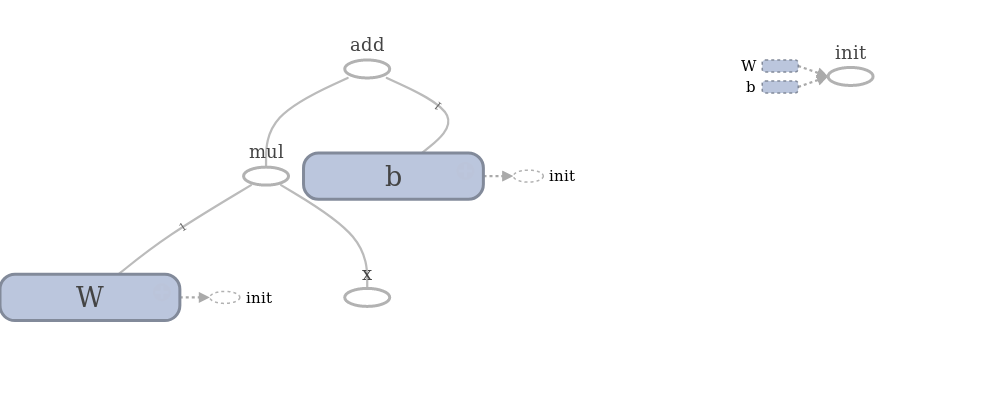
\includegraphics[width=10cm]{./figures/graphAddition.png} 
\end{center}
\caption{Graphe de calcul simple}
\end{figure}

On retrouve dans ce graphes la présence des deux variables ($W$ et $b$), le placeholder $x$, et un noeud $add$ dont la sortie correspond à $y$.


Par ailleurs, les variables au sens TensorFlow sont des nœuds de calculs qui peuvent être modifiés. Elle ne sont pas initialisées par leur déclaration. Il faudra explicitement demander leur initialisation pour qu'elles agissent comme on s'y attend.
Il s'agit maintenant pour que notre programme calcule bien la valeur voulue de :
\begin{itemize}
\item construire le graphe de calcul a partir des informations précédentes.
\item initialiser les variables $W$ et $b$
\item lancer le calcul de y avec une valeur choisie pour $x$...
\end{itemize}

Ajoutons les codes suivants à notre programme
\begin{mypython}
sess = tf.Session()
\end{mypython}
Le code ci-dessus construit le graphe.
\begin{mypython}
init = tf.global_variables_initializer()
sess.run(init)
\end{mypython}
Le code ci-dessus initialise toutes les variables du programme (W et b). En fait, ce code construit un noeud de calcul correspondant a l'initialisation (première ligne) et lance le calcul correspondant (deuxième ligne).

\begin{mypython} 
resu = sess.run(y, {x:2}) 
print(resu)
\end{mypython}
Ce code lance le calcul de y, en prenant soin de placer la valeur 2 dans le placeholder x et afficher le résultat attendu
\begin{myoutput}
[0.3]
\end{myoutput}
Pour comprendre l'intérêt de ces concepts de graphe de calcul, ajoutons à la fin de notre programme existant le code suivant :

\begin{mypython} 
resu = sess.run(y, {x:[1, 2, 3]}) 
print(resu)
\end{mypython} 

Cette fois ci, les sorties sont :

\begin{mypython} 
[0.3]
[0.  0.3 0.6]
\end{mypython} 

Nous avons en fait lancé deux runs (deux calculs de y). La première fois, x est un réel, la seconde fois x est un tableau de réels. Dans le second cas, pour chaque valeur de x, une valeur est calculée pour y.
Notre programme a donc mis en place une procédure de calcul (le graphe de calcul) que l'on peut utiliser de multiples fois, avec différentes valeurs d'entrées (qui de plus prennent des formes différentes).
Une grande partie de la force de TensorFlow tient dans ces notions.

Voici donc le code du programme complet. Ce code est contenu dans le fichier :\\
\verb+DNN/Documentation/TutosPython/PremiersCalculs/calculTensorFlow.py+

\lstinputlisting[style=generalFrame,backgroundcolor=\color{darkwhite}]{../../TutosPython/PremiersCalculs/calculTensorFlow.py}

\subsubsection{Formalisation des concepts}
Ceci tient en quelques mots :
\begin{itemize}
\item TensorFlow s'appuie sur un \textbf{graphe de calcul}.
\item Les nœuds de ce graphe sont des \textbf{opérations}.
\item Sur les arêtes de ce graphe circulent des \textbf{tenseurs}. Ces tenseurs sont les sorties des nœuds du graphe.
\item Faire des calculs avec TensorFlow, c'est lancer un run en demandant le calcul d'une de ces sorties.
\end{itemize}

\subsection{Premiers pas avec Tensorboard}

TensorBoard est l'outil de visualisation associé à TensorFlow. Il permet de visualiser le graphe de calcul, mais aussi des valeurs importantes retenues lors des calculs exécutés sur ce graphe de calcul.
Pour sélectionner les informations a visualiser, nous l'indiquerons a notre programme TensorFlow. Le programme sauvegardera ces informations dans un répertoire spécifique.

On pourra alors lancer l'exécutable TensorBoard qui va analyser ce répertoire, créer un serveur web local que l'on pourra consulter pour visualiser nos informations...
Voyons comment tout ceci se fait.


Ajout de code dans le programme TensorFlow (a la fin du programme précédent) :
\begin{mypython}
pathLog="./SaveHere/";
writer = tf.summary.FileWriter(pathLog, sess.graph)
writer.close()
\end{mypython}
Ici, on choisit le répertoire (répertoire de Log) dans lequel seront stockées les informations importantes, et on crée un objet permettant d'écrire les informations de notre programme sur le disque. Ici, nous ne sauvons que le graphe de calcul. Enfin, on ferme cet objet.

Le code du programme complet est contenu dans le fichier :\\
\verb+DNN/Documentation/TutosPython/PremiersCalculs/calculTensorFlowWithTensorBoard.py+

\lstinputlisting[style=generalFrame,backgroundcolor=\color{darkwhite}]{../../TutosPython/PremiersCalculs/calculTensorFlowWithTensorBoard.py}



On lance notre programme TensorFlow 
\begin{mybash}
python .\calculTensorFlowWithTensorBoard.py
\end{mybash}
On lance ensuite TensorBoard sur le répertoire de Log avec la ligne suivante :

\begin{mybash}
tensorboard --logdir=./SaveHere
\end{mybash}


L’exécution donne le message suivant :
\begin{myoutput}
Starting TensorBoard b'41' on port 6006
(You can navigate to http://127.0.1.1:6006)
\end{myoutput}


Enfin, on ouvre un navigateur dans lequel on indique l'URL de consultation indiquée par la sortie précédente.

Voici une capture de la visualisation obtenue :
\begin{figure}[H]

\begin{center}
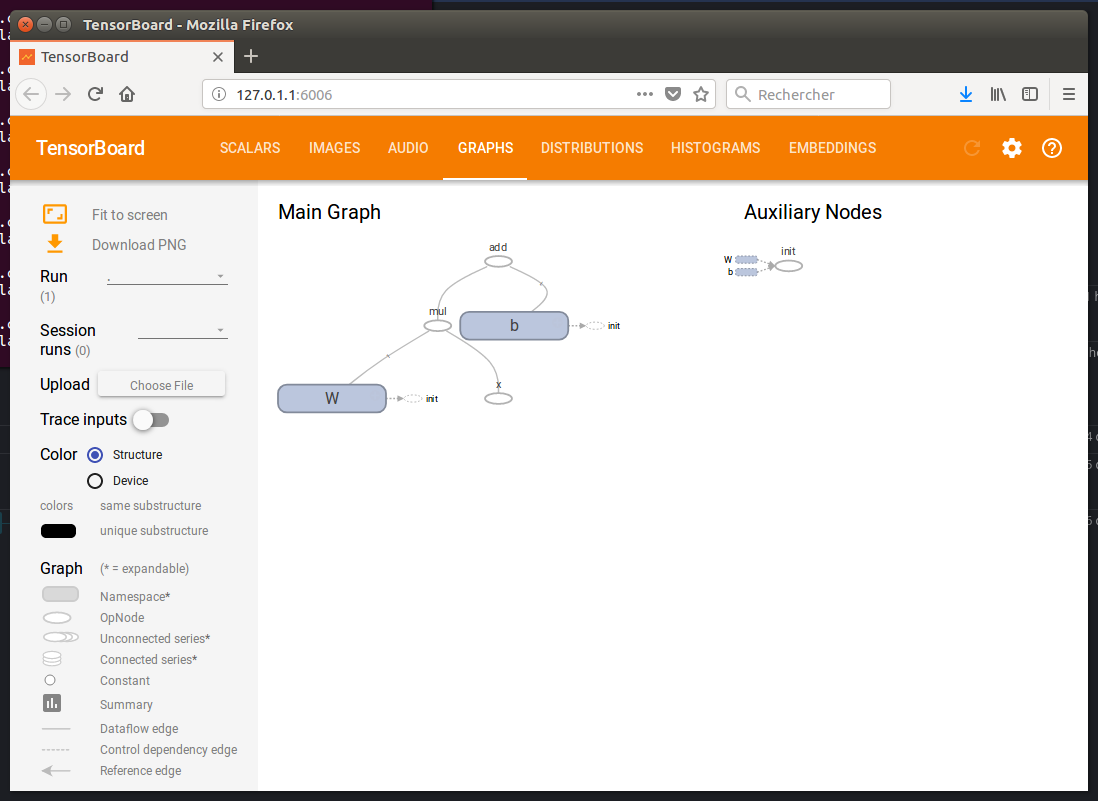
\includegraphics[width=10cm]{./figures/premierTensorBoard.png} 
\end{center}
\caption{La fenêtre de visualisation de TensorBoard}
\end{figure}

On retrouve ici le graphe précédent. Notez le sous graphe en haut a droite (noeud init) correspondant à l'initialisation des variables dont nous avons parlé précédemment.
On verra plus loin que TensorBoard nous permet aussi de visualiser l'évolution de nos apprentissages...

\chapter{Première Classification : Base IRIS}
Sur cette base comme pour les autres, nous allons considérer deux cas :
\begin{itemize}
\item on crée le classifieur manuellement (boite blanche)
\item on utilise un classifieur prédéfini (boite noire)
\end{itemize}

Cette base a 3 classes possibles et chaque exemple présente 4 caractéristiques.

\section{Reseau monocouche boite blanche}
Le code complet de ce programme sera donné en fin de section. Voyons quelques grandes étapes.

\subsection{lecture des données}

Supposons que les données soient déja présentes sur le disque, on les lira comme suit, par exemple pour la base d'apprentissage.

\begin{mypython}
# Load datasets.
training_set = tf.contrib.learn.datasets.base.load_csv_with_header(
  filename="training_set.csv",
  target_dtype=np.int,
  features_dtype=np.float32)
\end{mypython}

L'objet \verb+training_set+ a un champ \verb+data+ qui contient les paramètres des exemples et un champ \verb+ target+ qui contient les labels des classes.

\subsection{Construction du réseau}
\subsubsection{Les entrées}
On crée ensuite les placeholders pour entrer ces données:
X est bien de taille 4.  
\begin{mypython}
with tf.name_scope('X'):
	# entrées
	x = tf.placeholder(tf.float32, [None, 4], name = "X")

with tf.name_scope('Y_True'):
    # sorties voulues
    y_int = tf.placeholder(tf.uint8, [None], name = "Y_int")
    y_ = tf.one_hot(y_int, depth=3, name = "Y_True")

\end{mypython}
A noter que l'on crée ici un noeud \verb+y_+ qui transforme le label (entier) d'une classe en un \textbf{hot vector}.
Par exemple, le label 0 parmi 3 classes possibles se transforme en hot vecteur : \verb+[1,0,0]+\\

\subsubsection{Le modèle}
Définissons notre modèle : un réseau monocouche linéaire.
Nous avons 3 neurones de sortie (1 par classe).
Chaque neurone a 4 entrées (les 4 paramètres).
Nous avons 4 poids et 1 biais par neurone.
Le score calculé pour chaque classe est classique.
\begin{mypython}
# Le modèle
with tf.name_scope("Weights"):
	W = tf.Variable(tf.zeros([4, 3]),name ="W")

with tf.name_scope("Biases"):
	b = tf.Variable(tf.zeros([3]), name = "b")
	
with tf.name_scope("Score"):
	score = tf.matmul(x, W) + b
\end{mypython}
Les lignes de type \verb+with tf.name_scope("Score"):+ servent juste à regrouper certains nœuds pour la visualisation avec TensorBoard.

\subsubsection{optimisation du modèle}
Pour trouver les meilleurs poids $(W,b)$ du réseau, il nous faut : un critère à minimiser, et un algorithme de minimisation.


Le critère à minimiser sera pour nous \textbf{l'entropie croisée}.
Pour le calculer, nous transformons les scores de chaque sortie en une probabilité (fonction \verb+softmax+). On veut ensuite calculer une distance entre ce vecteur de probabilité et la distribution voulue (le hot vector d'entrée). L'entropie croisée fera office de distance.
\begin{mypython}
with tf.name_scope('softmax'):
	y = tf.nn.softmax(score)
with tf.name_scope('cross_entropy'):
	cross_entropy = tf.reduce_mean(-tf.reduce_sum(y_ * tf.log(y), reduction_indices=[1]))
\end{mypython}

Pour savoir quelle est la classe prédite il faut regarder quelle sortie a donné le plus fort score :
\begin{mypython}
classe = tf.argmax(y,1)    
\end{mypython}

Pour mesurer la précision (le taux de reconnaissance), il faut vérifier si la classe retenue pour un exemple est bien la classe donnée par la base. On calcule ensuite le taux moyen de succès sur un ensemble d'exemples :
\begin{mypython}
with tf.name_scope('Accuracy'):
	correct_prediction = tf.equal(tf.argmax(y,1), tf.argmax(y_,1))
	accuracy = tf.reduce_mean(tf.cast(correct_prediction, tf.float32))
\end{mypython}

On choisit enfin une méthode d'optimisation. Ici, une descente de gradient appliquée à notre entropie croisée.
\begin{mypython}
# Choix d'une méthode de minimisation
with tf.name_scope('train'):
	train_step = tf.train.GradientDescentOptimizer(0.5).minimize(cross_entropy)
\end{mypython}
Cette descente de gradient définit un nœud de calcul \verb+train_step+ que l'on pourra appeler lors du run.

\subsubsection{lancement des calculs}
On initialise tout d'abord les variables du réseau.
\begin{mypython}
init = tf.global_variables_initializer();
sess.run(init);
\end{mypython}

Apprentissage : On lance le run sur le noeud de calcul \verb+train_step+.
\begin{mypython}
for i in range(1000):
  sess.run(train_step, feed_dict={x: training_set.data, y_int: training_set.target})
\end{mypython}

Evaluons notre apprentissage sur la base d'apprentissage : On lance le run sur le noeud de calcul correspondant à la précision. 
\begin{mypython}
print("Resultats en Apprentissage", sess.run(accuracy, feed_dict={x: training_set.data, y_int: training_set.target}))
\end{mypython}

Voyons une prédiction : on lance le run sur le noeud de calcul de classe, avec des exemples inconnus.
\begin{mypython}
new_samples = np.array(
  [[6.9, 3.2, 4.5, 1.5],
   [4.8, 3.1, 5.0, 1.7]], dtype=np.float32)
  
print("classe ", sess.run(classe, {x: new_samples}))
\end{mypython}

A ce stade, nous avons un classifieur fonctionnel.
Ajoutons quelques améliorations pour la visualisation avec TensorBoard.

\subsection{TensorBoard : Evolution des performances}
Nous allons modifier notre code pour disposer de graphiques d'évolution de la précision et de l'entropie croisée au cours de l'apprentissage.

Commençons par choisir un répertoire, et ouvrons un \verb+FileWriter+ pour écrire dedans
\begin{mypython}
visuPath = './VisuMonoCouche'
writer = tf.summary.FileWriter(visuPath, sess.graph)
\end{mypython}

Signalons ensuite que nous voulons suivre l'entropie croisée et la précision. Ces infos seront fusionnées pour le \verb+FileWriter+ en un nœud \verb+merged+.
\begin{mypython}
tf.summary.scalar('Entropie Croisee', cross_entropy)
tf.summary.scalar('Precision', accuracy)

merged = tf.summary.merge_all()
\end{mypython}

L'apprentissage doit etre un peu modifié : Quand on lance un run d'apprentissage, on calcule aussi le noeud \verb+merged+. Sa sortie est récupérée dans la variable \verb+summary+. Celle ci est passée au \verb+FileWriter+ qui gère la sauvegarde.
\begin{mypython}
for i in range(1000):
  summary, _ = sess.run([merged,train_step], feed_dict={x: training_set.data, y_int: training_set.target})

  writer.add_summary(summary, i)
\end{mypython}

On peut améliorer un peu notre programme en téléchargeant la base IRIS si on ne l'a pas sur le disque, et effacer le répertoire de visualisation pour éviter qu'il ne se remplisse de données, ce qui donnerait le programme complet suivant contenu dans le fichier :\\
\verb+DNN/Documentation/TutosPython/Iris/irisMonocoucheComplet.py+

\lstinputlisting[style=generalFrame,backgroundcolor=\color{darkwhite}]{../../TutosPython/Iris/irisMonocoucheComplet.py}

\subsection{Sauvegarde et Chargement d'un réseau }




\section{ Classification de la base IRIS avec un DNN }
Nous  allons utiliser  tf.estimator  pour construire un classificateur de réseau neuronal et l'entraîner sur l' ensemble de données Iris pour prédire les espèces de fleurs basées sur la géométrie des sépales / pétales. Pour cet exemple  les données Iris ont été randomisées et divisées en deux CSV distincts:
\begin {itemize}
\item Un ensemble d'apprentissage de 120 échantillons ( \verb+iris_training.csv+ )
\item	Un ensemble de test de 30 échantillons ( \verb+iris_test.csv+ ).
\end{itemize}
 Voici les  codes pour construire le code complet  du classificateur de réseau neuronal:
\begin{mypython}
from __future__ import absolute_import
from __future__ import division
from __future__ import print_function

import os
from six.moves.urllib.request import urlopen

import numpy as np
import tensorflow as tf

# Data sets
IRIS_TRAINING = "iris_training.csv"
IRIS_TRAINING_URL = "http://download.tensorflow.org/data/iris_training.csv"

IRIS_TEST = "iris_test.csv"
IRIS_TEST_URL = "http://download.tensorflow.org/data/iris_test.csv"

def main():
  # If the training and test sets aren't stored locally, download them.
  if not os.path.exists(IRIS_TRAINING):
    raw = urlopen(IRIS_TRAINING_URL).read()
    with open(IRIS_TRAINING, "wb") as f:
      f.write(raw)

  if not os.path.exists(IRIS_TEST):
    raw = urlopen(IRIS_TEST_URL).read()
    with open(IRIS_TEST, "wb") as f:
      f.write(raw)
\end{mypython}
Le code ci-dessus importe  tous les modules nécessaires et définit où télécharger et stocker l'ensemble de données : les bases d'apprentissage et de généralisation s'ils ne sont pas stockés localement.
Ces bases sont au format \textbf{csv}.
\begin{mypython}
training_set = tf.contrib.learn.datasets.base.load_csv_with_header(
      filename=IRIS_TRAINING,
      target_dtype=np.int,
      features_dtype=np.float32)
test_set = tf.contrib.learn.datasets.base.load_csv_with_header(
      filename=IRIS_TEST,
      target_dtype=np.int,
      features_dtype=np.float32)
\end{mypython}
Le code ci-dessus charge en mémoire les bases d'apprentissage et de généralisation. Notons la fonction en utilisant la fonction \verb+tf.contrib.learn.datasets.base.load_csv_with_header+ qui permet de charger des fichiers \textbf{csv}.
\begin{mypython}
feature_columns = [tf.feature_column.numeric_column("x", shape=[4])]
\end{mypython}
Ce code prépare une variable pour les entrées du modèle (le vecteur de caractéristiques ou \textbf{feature vector}) et spécifie que \textbf{feature vector} est numériques et de dimension 4 (longueur des sépales, largeurs des sépales, longueur des pétales, largeur des pétales).

\begin{mypython}
classifier = tf.estimator.DNNClassifier(feature_columns=feature_columns,
                                          hidden_units=[10, 20, 10],
                                          n_classes=3,
                                          model_dir="/tmp/iris_model")
\end{mypython}
Ce code crée un Réseau de Neurones Profond (Deep Neural Network ou \textbf{DNN}) que l'on utilisera pour classifier nos données. Pour le construire on lui passe les informations suivantes :
\begin{itemize}
\item la forme du \textbf{feature vector}.
\item la topologie du réseau. Ici : trois couches cachées , contenant respectivement 10, 20 et 10 neurones.
\item le nombre de classes attendues en sortie. Ici : Trois classes, représentant les trois espèces d'Iris.
\item le répertoire dans lequel TensorFlow sauvegardera en particulier les données utilisées par  TensorBoard pour la visualisation.
\end{itemize}

Le code qui suit va lancer l'apprentissage. l'Estimator de TensorFlow impose la structure de code suivante :
\begin{itemize}
	\item on définit une fonction spécifiant :
	\begin{itemize}	
		\item le jeu de donnée utilisé (caractéristiques et labels).
		\item le nombre d'\textbf{epochs} lors de l'apprentissage.
		\item si les données doivent être présentées dans un ordre aléatoire
	\end{itemize}
	\item on lance l'entrainement qui utilise cette fonction un certain nombre de fois.
\end{itemize}
\begin{mypython}
train_input_fn = tf.estimator.inputs.numpy_input_fn(
      x={"x": np.array(training_set.data)},
      y=np.array(training_set.target),
      num_epochs=None,
      shuffle=True)

classifier.train(input_fn=train_input_fn, steps=2000)
\end{mypython}

On suit la même logique lorsqu'on veut évaluer le classifieur sur la base d'apprentissage, mais on lance cette fois la fonction d'évaluation du classifieur.
\begin{mypython}
train_input_eval_fn = tf.estimator.inputs.numpy_input_fn(
      x={"x": np.array(training_set.data)},
      y=np.array(training_set.target),
      num_epochs=1,
      shuffle=False)

  
accuracy_score = classifier.evaluate(input_fn=train_input_eval_fn)["accuracy"]
print("\nLearning Accuracy: {0:f}\n".format(accuracy_score))
\end{mypython}

Enfin, on évalue le classifieur sur la base de généralisation.
\begin{mypython}
test_input_fn = tf.estimator.inputs.numpy_input_fn(
      x={"x": np.array(test_set.data)},
      y=np.array(test_set.target),
      num_epochs=1,
      shuffle=False)
accuracy_score = classifier.evaluate(input_fn=test_input_fn)["accuracy"]
print("\nTest Accuracy: {0:f}\n".format(accuracy_score))
\end{mypython}

 
la sortie de ce programme donne quelque chose comme : soit une précision en généralisation de 0.97%.
\begin{myoutput}
Learning Accuracy: 1.000
Test Accuracy: 0.966667
\end{myoutput}


Si l'on souhaite prédire les classes de nouveaux exemples, on peut procéder comme suit en lançant la fonction de prédiction du classifieur, dont on affichera les résultats.

\begin{mypython}
new_samples = np.array(
      [[6.9, 3.2, 4.5, 1.5],
       [4.8, 3.1, 5.0, 1.7]], dtype=np.float32)

predict_input_fn = tf.estimator.inputs.numpy_input_fn(
      x={"x": new_samples},
      num_epochs=1,
      shuffle=False)

predictions = list(classifier.predict(input_fn=predict_input_fn))
  
for p in predictions :
    chaine =p["classes"]
    print ("classe ", chaine[0].decode()) 

\end{mypython}

La sortie du programme complet serait :
\begin{myoutput}
Learning Accuracy: 1.000000
Test Accuracy: 0.966667
classe  1
classe  2
\end{myoutput}

Ci dessous, les figures respectives de l'évolution des paramètres du réseau pendant l'apprentissage et du graphe de calcul.
\begin{figure}[H]

\begin{center}
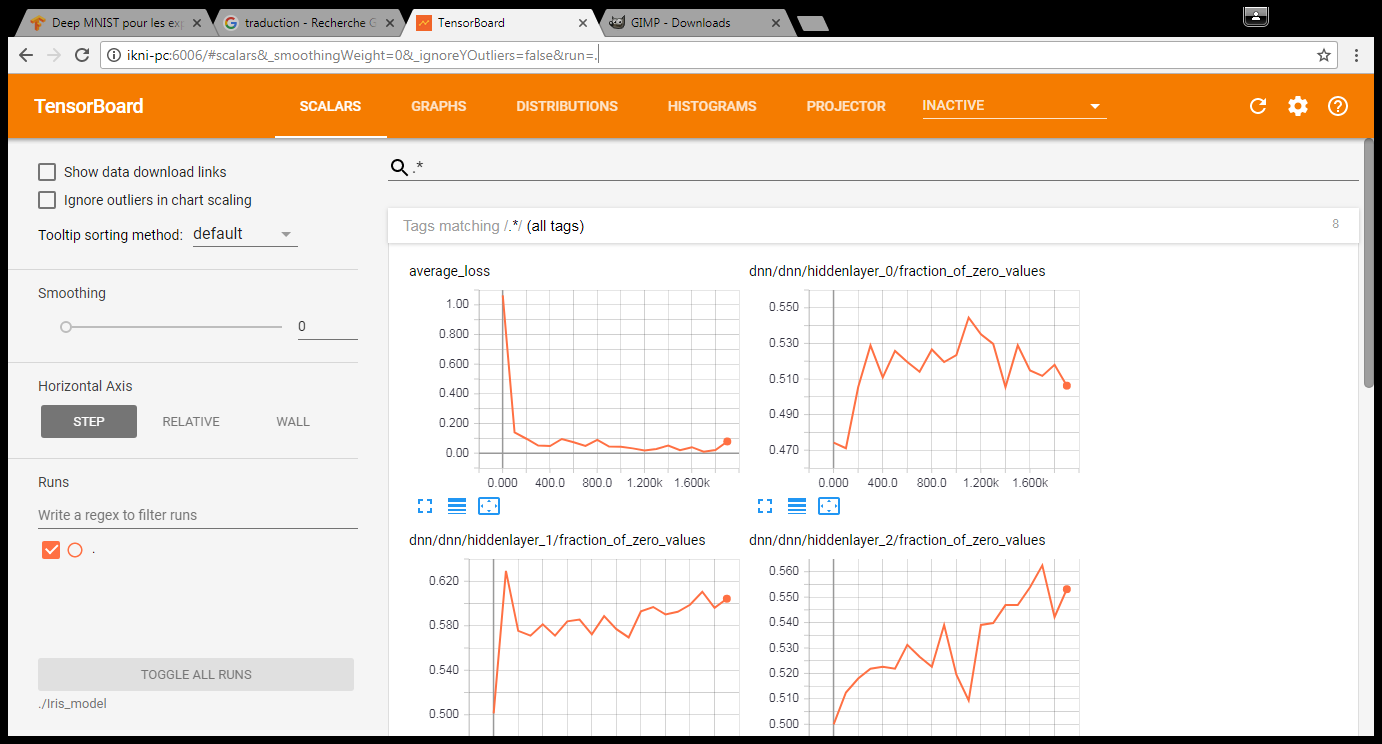
\includegraphics[width=16cm]{./figures/TensorBoardIrisDnn.png} 
\end{center}
\caption{Evolution des paramètres du réseau sur la base IRIS}
\end{figure}

\begin{figure}[H]

\begin{center}
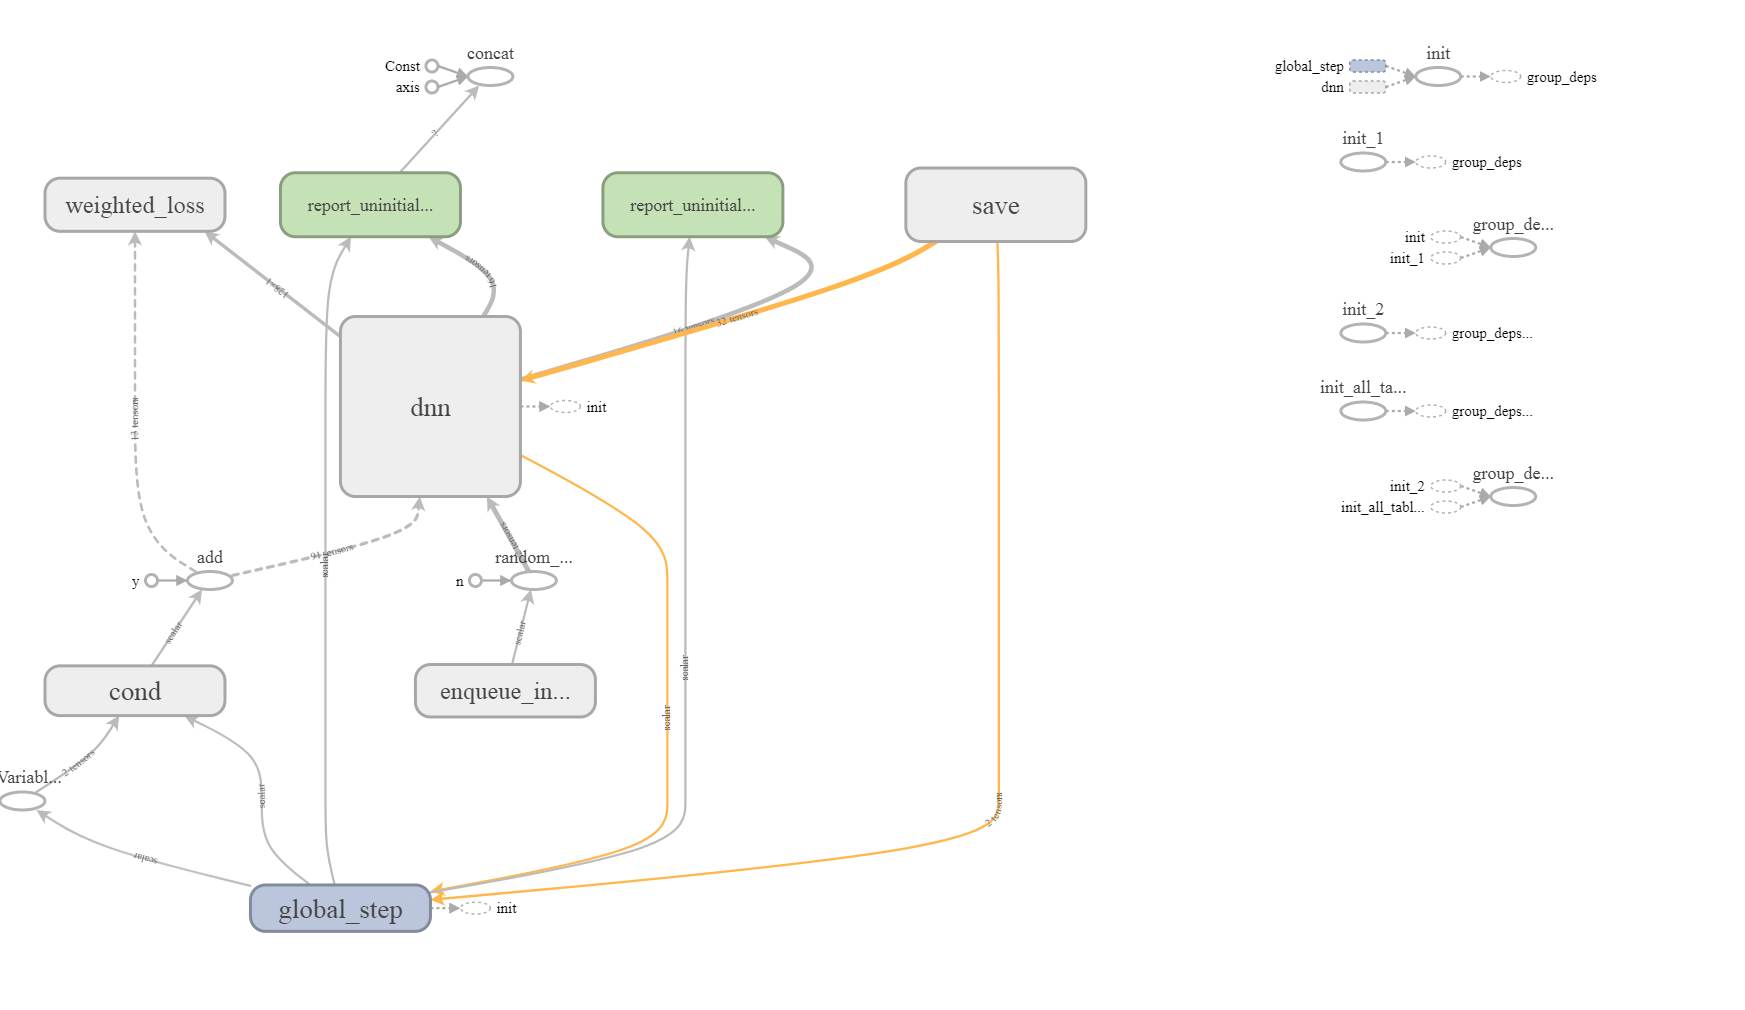
\includegraphics[width=10cm]{./figures/graphIrisDNN.png} 
\end{center}
\caption{Graphe de calcul du DNN utilisé sur la base IRIS}
\end{figure}

\chapter{bases MNIST et Fashion MNIST}
\section{MNIST}

\subsection{Récupération et chargement de la base MNIST}
\label{secGetMnist}
Lecture des données : Nous importons un module permettant de récupérer la base MNIST, puis on demande à ce module de lire les données. Si elles ne sont pas présentes, il va les télécharger sur le site de MNIST 
(\verb+http://yann.lecun.com/exdb/mnist/+)

\begin{mypython}
from tensorflow.examples.tutorials.mnist import input_data
mnist = input_data.read_data_sets("MNIST_data/", one_hot=True)
\end{mypython}

\subsection{Réseau Linéaire monocouche}
\subsubsection{Modèle du Réseau Linéaire monocouche}
\label{secMnistMono}

On utilisera ici un modèle purement linéaire contenant une couche de 10 neurones (c'est la couche de sortie).
 
\begin{mypython}
# entrées
x = tf.placeholder(tf.float32, [None, 784])

# sorties voulues
y_ = tf.placeholder(tf.float32, [None, 10])

# Le modèle
W = tf.Variable(tf.zeros([784, 10]))
b = tf.Variable(tf.zeros([10]))

# sorties calcules 
score = tf.matmul(x, W) + b
\end{mypython}

Pour l'apprentissage des poids $(W,b)$, on utilisera comme critère à minimiser l'entropie croisée.
Pour cela, la sortie de chaque neurone est transformée en probabilité avec la méthode \verb+softmax+.
Puis on calcule l'entropie croisée entre cette distribution de probabilité et la distribution de probabilité voulue.
\begin{mypython}
y = tf.nn.softmax(score)
cross_entropy = tf.reduce_mean(-tf.reduce_sum(y_ * tf.log(y), 	reduction_indices=[1]))
\end{mypython}

Pour le calcul de la précision, voici le code
\begin{mypython}
correct_prediction = tf.equal(tf.argmax(y,1), tf.argmax(y_,1))
accuracy = tf.reduce_mean(tf.cast(correct_prediction, tf.float32))
\end{mypython}

La partie apprentissage et évaluation sur les deux bases est classique...
\begin{mypython}
# Apprentissage
for i in range(1000):
  batch_xs, batch_ys = mnist.train.next_batch(100)
  sess.run(train_step, feed_dict={x: batch_xs, y_: batch_ys})

# Evaluation
print("Resultats en Apprentissage", sess.run(accuracy, feed_dict={x: mnist.train.images, 	y_: mnist.train.labels}))
print("Résultats en Généralisation", sess.run(accuracy, feed_dict={x: mnist.test.images, 	y_: mnist.test.labels}))
\end{mypython}

\subsubsection{Code complet du réseau linéaire monocouche}
Le code complet, incluant des instructions de mise en forme pour TensorBoard est le suivant. Ce code est contenu dans le fichier :\\
\verb+DNN/Documentation/TutosPython/Mnist/mnistMonocoucheComplet.py+

\lstinputlisting[style=generalFrame,backgroundcolor=\color{darkwhite}]{../../TutosPython/Mnist/mnistMonocoucheComplet.py}


\subsubsection{Performances du réseau linéaire monocouche}
\label{secPerfMnistMono}
Pour information, voici des performances standard obtenues sur la base MNIST.
\begin{myoutput}
Résultats en Apprentissage 0.91827273
Résultats en Généralisation 0.9178
\end{myoutput}

\subsection{DNN Multicouches}
\subsubsection{Modèle du Réseau de neurones multicouches}
\label{secMnistMulti}

Ici, un réseau à deux couches, avec Estimator.


\section{Fashion MNIST}

La base Fashion MNIST ressemble beaucoup à la base MNIST :
\begin{itemize}
\item Même nombre d'entrées
\item Même nombre de classes
\item Même nombre d'exemples
\item Même noms de fichiers
\end{itemize}
De ce fait, nous pouvons utiliser les mêmes procédures pour charger les exemples que celle utilisées pour MNIST. Ces procédures font partie du module exemple de tensorflow que l'on charge comme suit :
\begin{mypython}
from tensorflow.examples.tutorials.mnist import input_data
\end{mypython}
La seule modification effective consiste a spécifier le répertoire ou l'on trouve les fichiers de Fashion MNIST :
\begin{mypython}
# Import data
fashionMnist = input_data.read_data_sets('./FM_DATA/', one_hot=True)
\end{mypython}
C'est cet objet \verb+fashionMnist+ qui fournira les données et les labels lors de l'entrainement et de l'évaluation.

\textbf{ATTENTION :} Nous utilisons içi un module conçu pour MNIST pour lire les données de Fashion MNIST. Conformément à ce qui a été dit dans la section~\ref{secGetMnist}, si le répertoire \verb+./FM_DATA/+ est vide ou n'existe pas, ce module va télécharger la base MNIST dedans !
Le téléchargement de Fashion MNIST doit donc être fait manuellement, depuis \verb+https://github.com/zalandoresearch/fashion-mnist/+.

\subsection{Réseau Linéaire monocouche}
\subsubsection{Principe et code complet du réseau linéaire monocouche}
\label{secFashionMnistMono}
Compte tenu de ce qui a été dit plus haut, le code est quasiment le même que dans le cas de MNIST vu dans la section \ref{secMnistMono}. 
Voici donc le code complet du programme. Ce code est contenu dans le fichier :\\
\verb+DNN/Documentation/TutosPython/FashionMNIST/fmnistMonocoucheComplet.py+

\lstinputlisting[style=generalFrame,backgroundcolor=\color{darkwhite}]{../../TutosPython/FashionMNIST/fmnistMonocoucheComplet.py}


\subsubsection{Performances du réseau linéaire monocouche}
\label{secPerfFMnistMono}

Voici ses performances
\begin{myoutput}
Résultats en Apprentissage 0.84214544
Résultats en Généralisation 0.8273
\end{myoutput}
avec une grande variabilité, car on peut aussi obtenir ceci :
\begin{myoutput}
Résultats en Apprentissage 0.7074182
Résultats en Généralisation 0.6953
\end{myoutput}

On peut noter la baisse de performances par rapport à ce qui était obtenu avec la base MNIST dans la section ~\ref{secPerfMnistMono}.

Selon l'évolution des performances ci-dessous, le réseau monocouche a atteint ses limites.

\begin{figure}[H]
\begin{center}
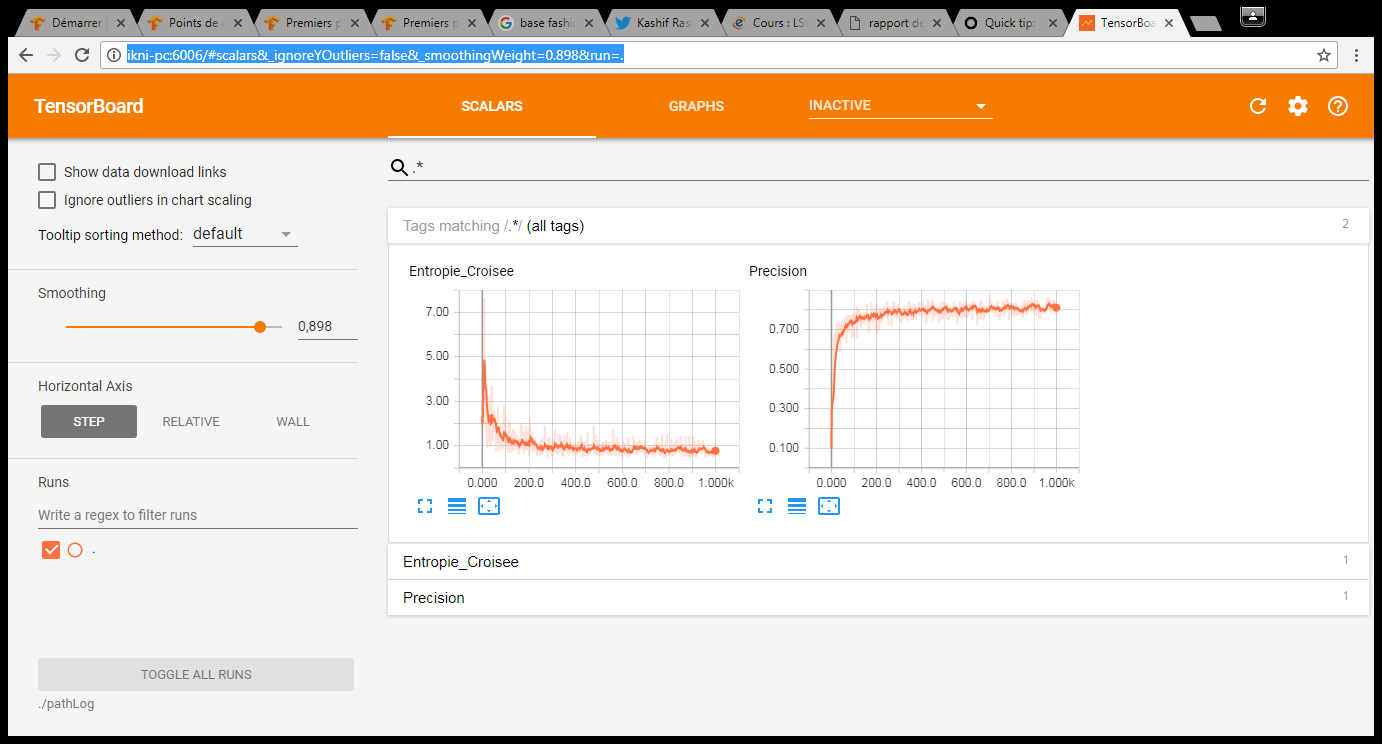
\includegraphics[width=15cm]{./figures/scalarFMnistMono.png} 
\end{center}
\caption{Évolution des performances en apprentissage}
\end{figure}


\end{document}
